\documentclass[11pt,a4paper]{article}
\usepackage[utf8]{inputenc}
\usepackage{amsmath}
\usepackage{amsfonts}
\usepackage{amssymb}
\usepackage{enumerate}
\usepackage{graphicx}
\usepackage{float,xcolor,fancyvrb,wrapfig}
\renewcommand{\labelitemi}{$-$}
\renewcommand*\footnoterule{\hrule}
\newcommand{\todo}[1]{{\color{blue} \texttt{\textbf{TODO.}} #1}}
\newcommand{\resitem}[1]{\item #1 \vspace{-7pt}}

\DeclareMathOperator*{\argmin}{arg\,min}
\usepackage[left=1.2in,right=1.2in,top=1in,bottom=1in]{geometry}
%\usepackage{fancyhdr}
%\pagestyle{fancy}

\newcommand{\sgr}{S_\text{gr}}
\newcommand{\sopt}{S_\text{opt}}

\usepackage{enumerate}

% Document header
% More info on customizing the layout: http://bit.ly/yEt7ny
%\lhead{Masters Project} % left
%\chead{} % center
%\rhead{Prabu {\sc Dhakshinamurthy}}

\begin{document}

\title{\bf Reorganizing DNS Log Data for Faster Querying and Optimizing Resource Usage on a Hadoop Cluster}
\author{
	\bf Prabu Dhakshinamurthy\\
	\textit{pdhakshi@cs.ucsd.edu}\\
	Masters Student\\
	University of California San Diego
}
\date {}
\maketitle

\begin{abstract} 
\noindent
Log data from DNS resolvers contain rich information that is quite useful for various research use cases such as estimating the popularity of websites. Log data from approximately 39k resolvers has been collected and stored on HDFS. The data is so huge and not optimally organized that it takes a lot of time and resources to search records of interest from the the log. In this project, we investigate techniques to port the log data to a new format so that it speeds up the query time and takes less resources both to store the data and to query the data. We investigated bzip compression, reformatting/pruning unessential records and partitioning the records into separate buckets and from our experiments, we found that using a combination of reformatting/pruning records with partitioning and efficiently sorting the records based on multiple fields speeds up the domain query by 6x and takes approximately 8x less resources to query in comparison with unorganized data. Also, the new data takes about 9x less space on disk.
\end{abstract} 

\section {Introduction}
Domain Name System (DNS) helps in identifying the internet resources such as finding the IP address of a host name, finding the host name of a given IP address, finding the mail server for a given domain and so on. Typically, end nodes send the translation requests to a local recursive resolver and the resolver queries the DNS. At the recursive resolver, the details about translation request(s)/response(s) are recorded in a log and this log data contains rich information about the access patterns of URLs by users in the network and it is being used in various researches such as estimating the popularity of websites\cite{peekingcloud}, identifying the IP addresses used by bad domains over a period of time and so on.
\\\\
A common query that users make over the log data is to filter the log records that match a particular domain(s) of interest. As of today, the raw log data stored on HDFS is not optimally structured to facilitate these queries and the data is so huge (in order of TBs per month) that it takes a lot of time and lot of resources like compute time, disk accesses and network usage to query the data. The query turnaround time gets even worse when the cluster is shared by multiple people at the same time.
\\\\
The goal of the project is to re-organize the log data to improve the query time of common domain based queries and reduce the resource usage to a significant extent. The rest of the report is organized as follows. Section 2 gives a background on the DNS resolution process. Section 3 outlines the DNS logging process and details the current log record format. Section 4 discusses the various techniques considered to optimize query and resource usage. Section 5 presents the experiment results and compares the performance of each of the techniques with the base line data. Section 6 shows a helper tool \textit{FindPartition} that users can use to query the log data. Section 7 discusses the future work and Section 8 summarizes and concludes the report.

\paragraph{Notations:} \textit{raw data: }Current log data; \textit{new data: }The new log data obtained by porting the raw data using a porting technique.

\section {Background on DNS resolution process}
DNS resolution is the process of identifying the internet resources such as IP address, hostname, mail server information and so on. For example, when a end-user types a URL in a browser, the browser contacts a DNS Resolver with an \texttt{A} type query, gets the IP address of the typed URL and then connects to the IP address obtained.
\\\\  
A typical iterative DNS resolution of a hostname to an IP address works as follows:
\begin{enumerate}
    \resitem {Client computer makes a DNS request to DNS Resolver to resolve a hostname to an IP address.}
    \resitem {Resolver responds with the IP address if it already has the resolution in it's cache.}
    \resitem {Otherwise, the resolver contacts the root name server (.) and gets the name server responsible for the TLD of the hostname being requested and contacts the corresponding name server.}
    \resitem {The TLD nameserver responds with another nameserver to contact and the resolver contacts that server.}
    \resitem {This iterative process is repeated until the resolver contacts an authoritative name server (which is authoritative for the domain and knows the IP address of the host name being requested) in which case, the authoritative server responds with the required hostname to IP address mapping.}
    \resitem {Once the DNS resolver receives the mapping, it caches the entry in its local cache and responds to the client. How long a DNS record is retained in the cache depends on Time To Live (TTL) of the domain and it is configured by the domain administrator.}
\end{enumerate}

The Figure below shows the various steps in the resolution process.
\begin{figure}[H] 
\centering
\includegraphics[width=0.55\textwidth]{./data/RESULTS/graphs/dns_resolution.png}
\caption {\textit{Iterative DNS Resolution Process.}}
\label{dns}
\end{figure}

\section {Data collection and Log Record format}
The log data from approximately 39k DNS resolvers is being collected for the past 22 months from ISC SIE framework\footnote{Security Information Exchange (SIE) is a private framework for information sharing in the Internet Security field and it allows participants to access the data on a subscription basis.}\cite{siedata} and stored on Hadoop Distributed File System (HDFS) located in UCSD. A log entry is made for every request that the DNS resolver makes to other DNS resolvers/name servers during an iterative name resolution process (in Figure \ref{dns}, a log entry is made for each pair of request/response that crosses the red line i.e., $<$2,3$>$, $<$4,5$>$ and $<$6,7$>$). If the address resolution is served from the local cache of the DNS resolver, then no log entry is made for that request. At present, the log data (from all the resolvers) for every 5 minute window (wall clock time) is collected and stored in a separate file on HDFS.

\subsection{Log Record Format}

A typical response from a DNS server contains the following sections and all three sections can be empty.
\begin{itemize}
	\resitem {Answer section: This section contains the answer desired i.e., the hostname to IP address mapping in case of A type queries.}
	\resitem {Authoritative section: This section lists the nameserver(s) which are authoritative for the requested domain.}
	\resitem {Additional section: This section contains additional information that may be helpful during the iterative process of the resolution process. For example, this section may identify the IP address of the authoritative nameservers of the requested domain.}
\end{itemize}
\noindent
A log record (a single line) stored on HDFS has the following comma separated fields:

\begin{table}[H]
\begin{tabular}{rp{0.8\linewidth}} \hline
\textbf{Field}      & \textbf{Description}\\
\hline
ts                 & Timestamp of the event that the log record marks.\\
type               & Type of UDP packet (query response, unanswered query etc).\\
src\_ip            & IP address of the recursive resolver that makes the request. In Figure \ref{dns}, it is the IP address of \textit{Recursive Resolver}.\\
dst\_ip            & IP address of the DNS server that the source resolver contacts. In Figure \ref{dns}, it corresponds to the IP addresses of name servers \textit{root, .com and Google}.\\
domain             & The domain/host name that is being resolved.\\
query\_type        & Type of query (\texttt{A, AAAA, PTR} etc).\\
rcode              & Return code of \textit{dig} command as contained in the response header.\\
answer\_count      & An integer representing the total number of answers that follows.\\
answer             & A list of $n$ answers of length $answer\_count$.\\
auth\_count        & An integer representing the total number of authoritative entries that follows.\\
authoritative      & A list of $n$ authoritative entries of length $auth\_count$.\\
adnl\_count        & An integer representing the total number of additional entries that follows.\\
additional         & A list of $n$ additional entries of length $adnl\_count$.\\

\end{tabular}
\end{table}

\newpage
\noindent
Example record:
\begin{verbatim}
1328083681,0,68.105.29.173,157.166.224.169,www.cnn.com.,1,0,4,5,
                         www.cnn.com.,150,IN,A,157.166.255.19,5,
                         www.cnn.com.,150,IN,A,157.166.226.25,5,
                         www.cnn.com.,150,IN,A,157.166.226.26,5,
                         www.cnn.com.,150,IN,A,157.166.255.18,0,0
\end{verbatim}

\subsection{Drawbacks of current log data organization}
As people query the log data for various research purposes, one common query that is observed on a daily basis is to filter all the log records that match domain(s) of interest and has query type $A$ (hostname to IP address mapping). As of today, the data is not organized in any particular fashion to optimize these queries.
\\\\
A user who wants to filter records matching domain \texttt{foo.com} in a day, has to sift through the entire day long log data which is about 30-40 GB. If \texttt{foo.com} appears only in few thousand records, then searching the entire day worth of log data is pure waste of resources (disk access, CPU usage, network bandwidth) and it takes more time on wall clock as well. So there is an opportunity to restructure the data and thereby reduce the query time/resource usage.
\\\\
The format of each record is not easy to follow and it takes a huge amount of disk space. So it is necessary to clean up the record, retain only fields of interest in a much more cleaner way and discard the other fields.

\section {Data restructuring}
The goal of the project is to improve the query time and to save the resources used. With this goal in mind, we tried the following techniques and each of them are discussed in detail in respective sections.
\begin{enumerate}

	\resitem {\textbf{Change compression format:} Use bz2 compression instead of gzip compression to store the data.}    \resitem {\textbf{Partition data:} Distribute the log records to multiple small sized buckets based on multiple parameters and thereby reduce the search space.}
    \resitem {\textbf{Reformat/Prune unessential records:} Simplify the format of a single record and remove unessential records.}
\end{enumerate}

\subsection{Change compression format}
Currently, the log data is compressed in gzip format and stored on disk. Bz2 compression is better than gzip in terms of the compression ratio and since bz2 compression is supported by Pig/Hadoop, it is worth trying to compress the log data using bz2 compression and assess the resource savings.

\subsection{Partition data}
A straightforward and simpler approach to organize the data in order to speedup the query would be to distribute the records into multiple buckets based on the hashcode of the domain (each record contains a domain field) and thus reduce the search space. But as the number of domains in the search query increases, it is possible that the domains span all the buckets and hence the search space remains same as before (entire data). So it is necessary to consider other parameters as well to organize the data.

\subsubsection{Record distribution}
As stated earlier in the report, a common query is to filter all the log records that match a domain(s) of interest and has query type $A$. Based on the observation, we estimated the distribution of the TLDs and the query type in the log records.

\begin{figure}[h] 
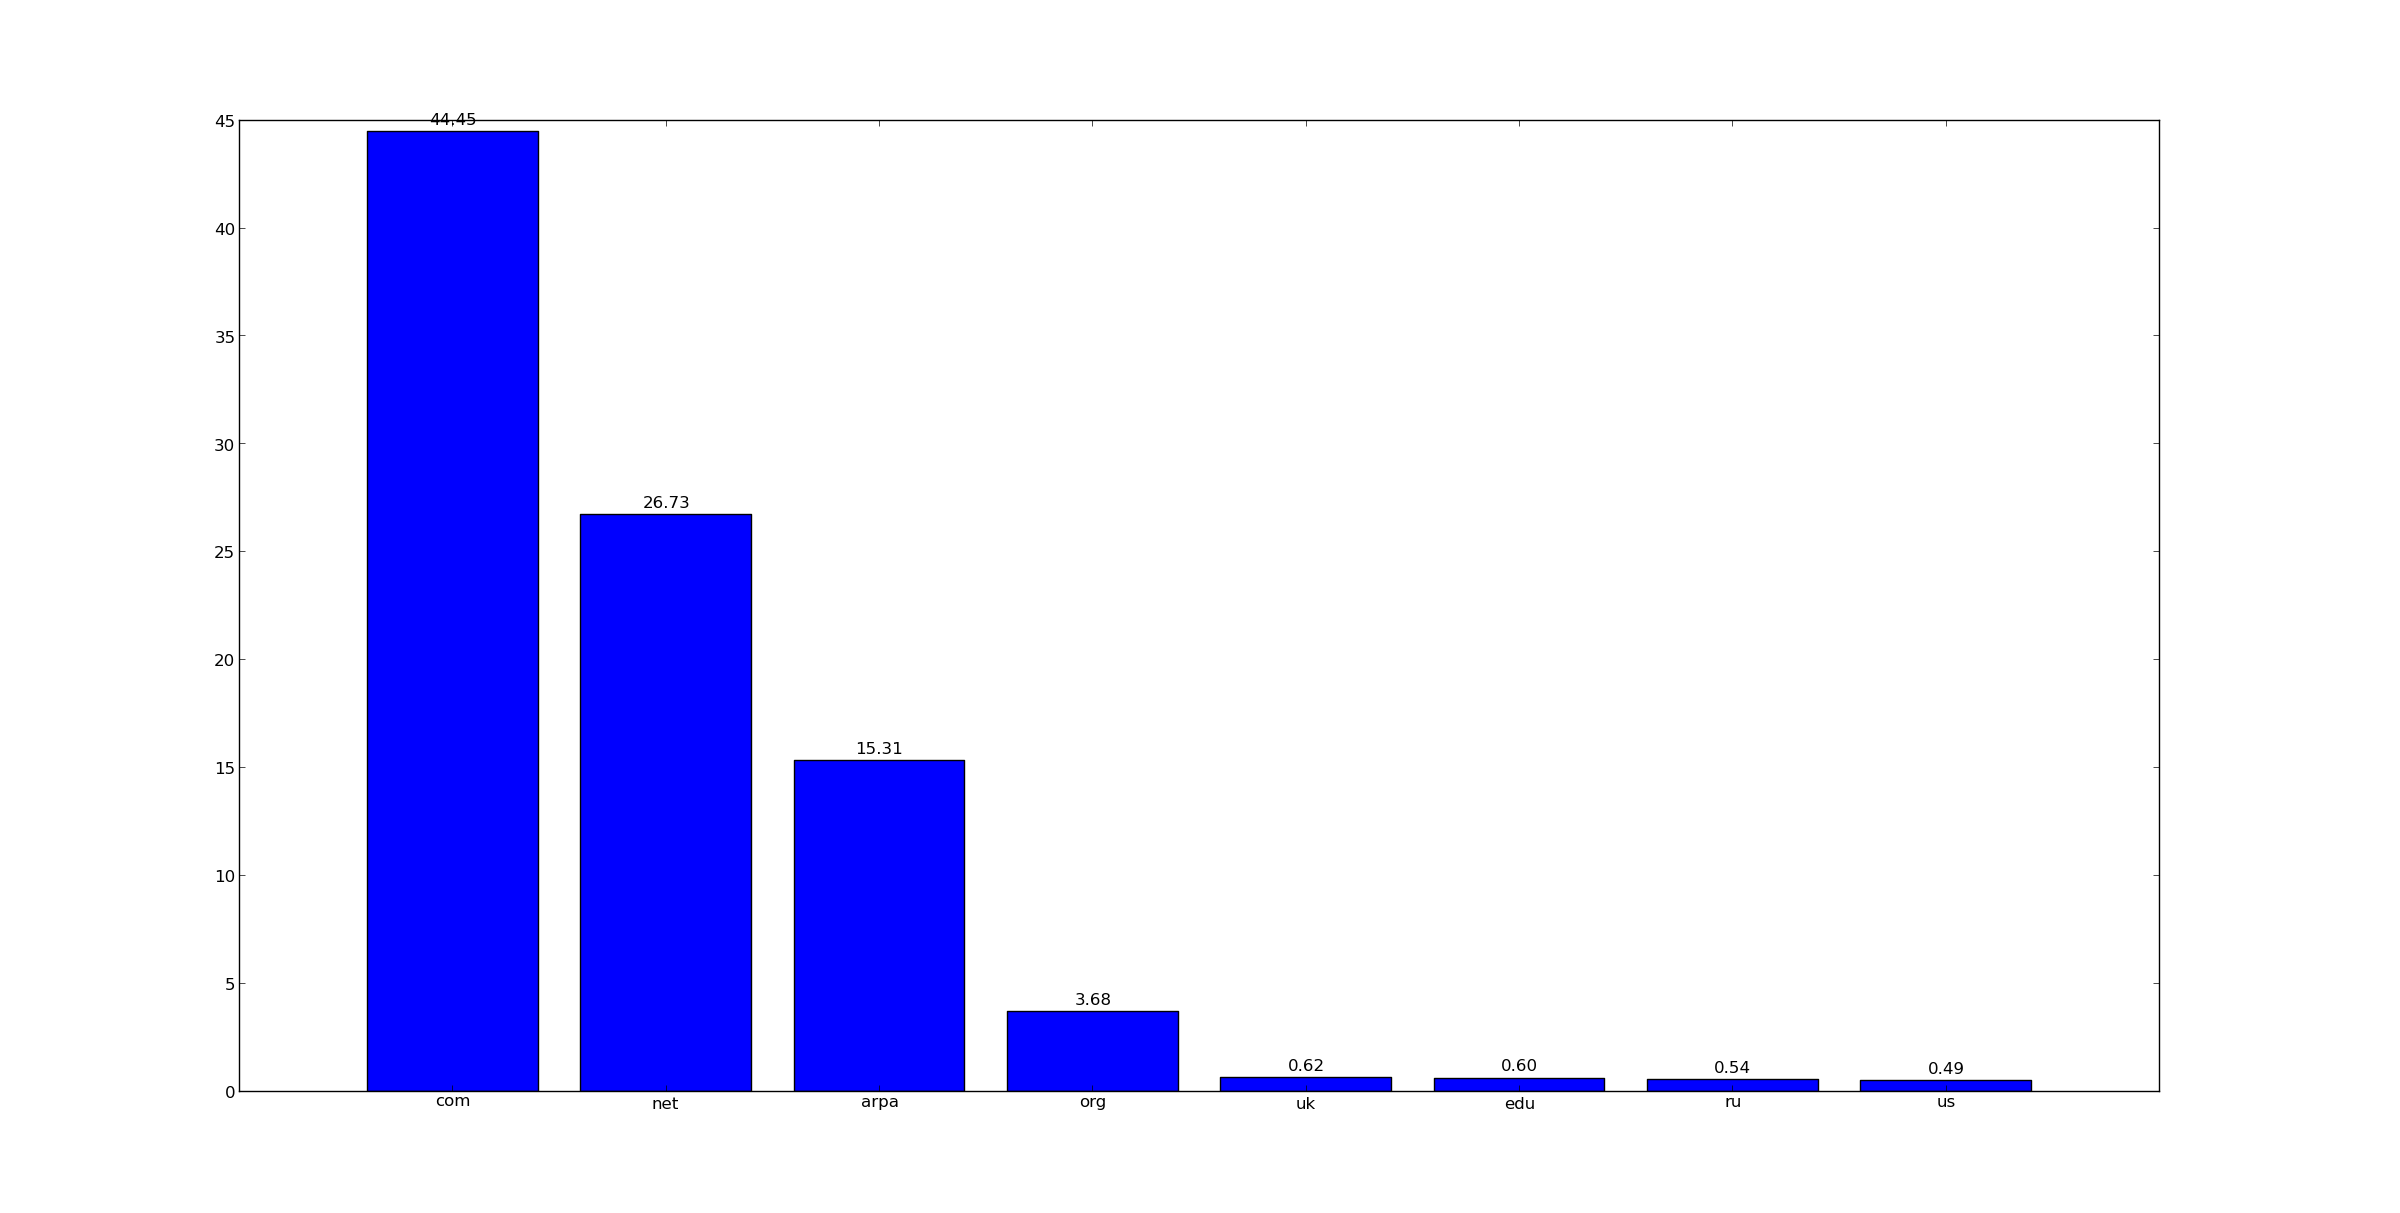
\includegraphics[width=1\linewidth]{./data/RESULTS/graphs/tld_distribution.png}
\caption {\textit{Distribution of log records by TLD.}}
\end{figure}

\begin{figure}[H] 
\centering
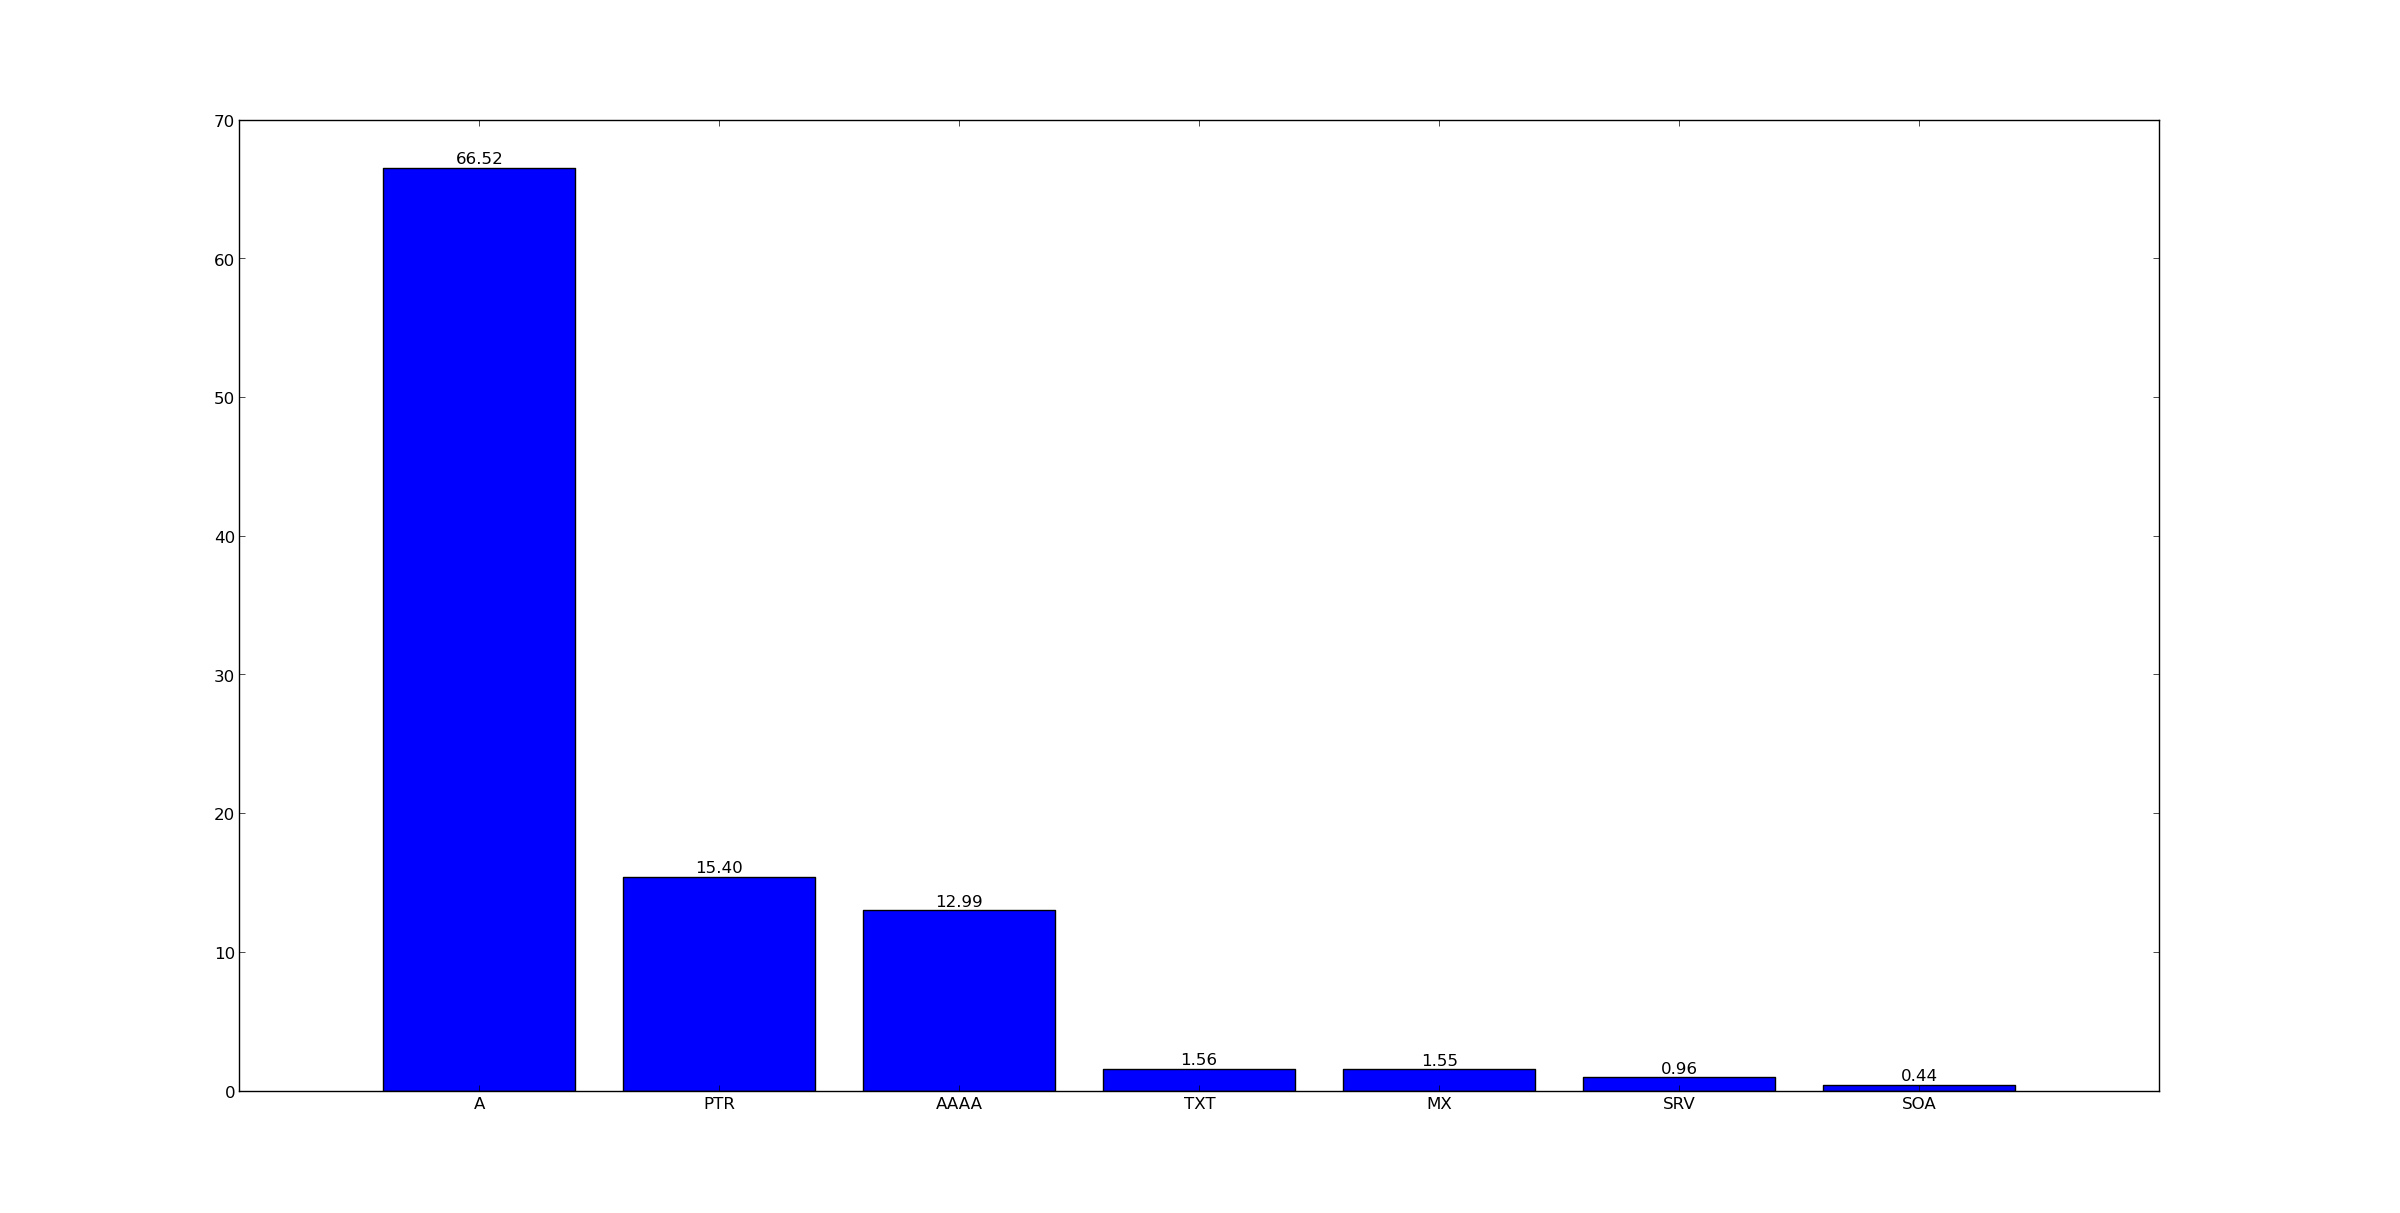
\includegraphics[width=1\textwidth]{./data/RESULTS/graphs/qtype_distribution.png}
\caption {\textit{Distribution of log records by query type.}}
\end{figure}

\noindent
Based on the TLD distribution above, it is clear that TLDs \texttt{com, net, arpa\footnote{arpa TLD is used for reverse dns look up i.e., given an IP address like 192.0.2.25, it is transformed as a name `25.2.0.192.in-addr.arpa' and then regular DNS resolution for this name is done with query type PTR to get the host name corresponding to the IP address.} and org} together constitute $87\%$ of the total records and the remaining $13\%$ is covered by all other TLDs. Similarly, the query type distribution chart shows that, query types \texttt{A, PTR and AAAA} are more prominent and covers $95\%$ of the total log records and other query types cover the remaining $5\%$ of the records. Osterweil et al.\cite{toptalker} had done similar estimation of the distribution of query types among \texttt{.com/.net} name servers; considering only the \texttt{.com/.net} domains, the relative query type distribution that we present here is in line with the numbers that Osterweil et al. reported.
\\\\
Since the user can query for a record by specifying the domain and the query type, it will be useful to study the combined distribution of TLDs and query type record. While finding the combined distribution, we take the top four TLDs as it is and we group all other TLDs into one single group and call it as a single TLD \texttt{OTHR}. Similarly, we take the top three query types as it is and tag all other query types as \texttt{OTHR}. So the TLD-querytype combination has twenty possibilities and the distribution of the records looks as below.

\begin{figure}[H] 
\centering
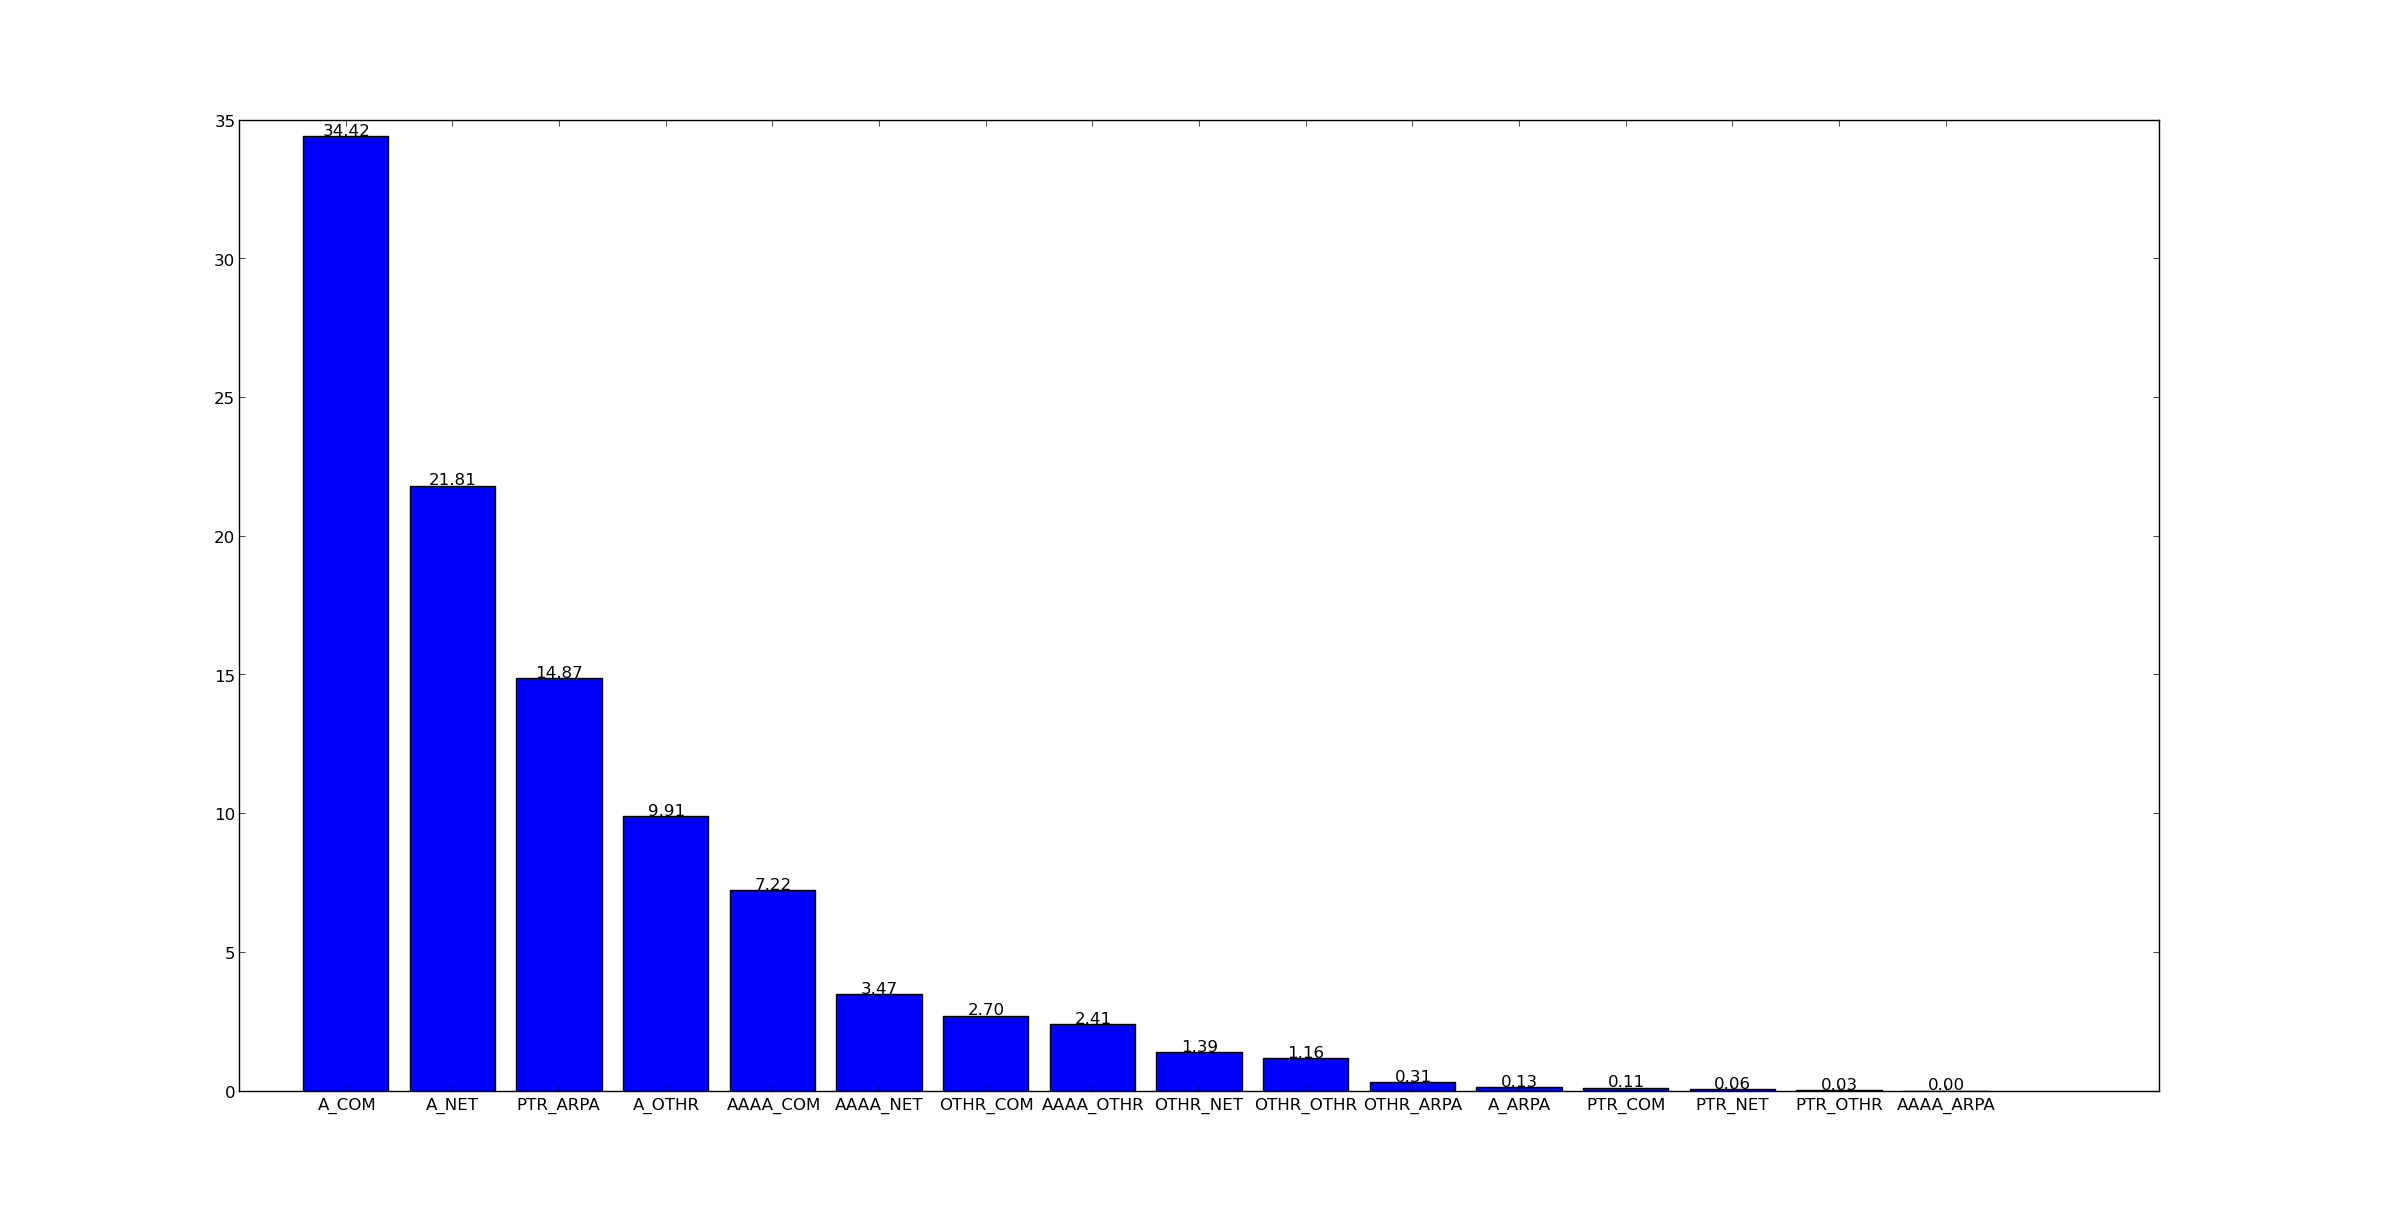
\includegraphics[width=1\textwidth]{./data/RESULTS/graphs/qtype_tld_dist.png}
\caption {\textit{Distribution of log records by query type and TLD.}}
\end{figure}

\noindent
From the TLD query type distribution, partitioning the log records into the $20$ buckets should help target the search queries to specific buckets thus reducing the search space and the query time. We term these $20$ buckets as $1^{st}$ level buckets for further discussion. Based on the use cases, we observed that people query the log data in the granularity of days. So we decided to support day level granularity after porting the data.
\\\\
The idea of partitioning each day log data into multiple buckets based on the query type and TLD can be represented as a data cube as shown below.
\begin{figure}[H] 
\centering
\includegraphics[width=0.55\linewidth]{./data/RESULTS/graphs/cube.png}
\caption {\textit{Visualization of qtype-TLD based partitioning of data over days.}}
\label{cube}
\end{figure}

\noindent
Then, the search space for a domain query with a query type filter in a given date range would be a sub-cube as highlighted (red cube) in Figure \ref{cube} for a \texttt{.com/A} query over Day1 data.
\\\\
Since the goal is to reduce the search space for the queries, creating smaller buckets within each of the $1^{st}$ level buckets will further reduce the bucket size. Bringing in the simpler idea of partitioning records based on the hashcode of the domains, all the records which fall into a particular $1^{st}$ level bucket are further hashed into $n$ smaller buckets termed $2^{nd}$ level buckets. The number of $2^{nd}$ level buckets $n$ within each $1^{st}$ level bucket is determined by the relative distribution of the records among the $1^{st}$ level buckets; for instance, A\_NET has thrice as many $2^{nd}$ level buckets as AAAA\_COM.
\\\\
The idea of having two levels of partitioning is motivated by domain queries of varying size (\#domains in the query). For \textit{single query} (only one domain), hashcode based partitioning is sufficient to reduce the search space. For \textit{small queries} (tens of domains) with mixed TLDs, hashcode partitioning helps to reduce the search space within each TLD buckets. For \textit{medium queries} (100-200 domains), it is likely that more domains will have the same TLD and based on their hashvalue, they will likely span all the $2^{nd}$ level buckets within a TLD bucket. So in this case, TLD based $1^{st}$ level partitioning helps to reduce the search space. For \textit{large queries} (1000s of domains), it is very likely that the domains span all TLD buckets and span all the hash buckets within each TLD and hence the search space will not reduce.

\subsubsection{Implementation Details}
The total number of buckets for a day worth of data is determined experimentally. While it seems obvious to have a large number of buckets in order to reduce the individual bucket size as much possible, on the HDFS environment it is not advisable to create lots of small files because,
\begin{itemize}
    \item {With millions of smaller files, namenode becomes heavy to maintain the metadata.}
    \resitem {For each smaller file, a separate map task is launched and the overhead of setting up the map task (setting up JVM) will be much higher than the useful work done and hence, the total job time increases.}
    \resitem {Map-Reduce environment has a limit on the maximum number of open files at a time and hence, creating lots of smaller buckets while porting the data will hit the open file limit.}
    \resitem {Files which are much smaller than HDFS block size (128MB) still need 1 HDFS block at the time of creation and hence the HDFS may complain about disk space.}
\end{itemize}

\noindent
Experimentally, a total of $200$ buckets per day results in average  bucket size of 30MB and also significantly reduces the search space for domain queries. For a total of 200 buckets, Figure \ref{doms} illustrates the number of buckets that will be searched as the number of domains in the search query increases for different domain sets and query type filter set to either \texttt{A} or \texttt{ALL}.

\begin{figure}[H] 
\centering
\includegraphics[width=0.8\linewidth]{./data/RESULTS/graphs/domain_vs_numbuckets.png}
\caption {\textit{\#Domains queried Vs \#Buckets searched.}}
\label{doms}
\end{figure}

\noindent
In all four types of queries, when the number of domains is lesser, the \#buckets searched is also lesser. But as the \#domains increase, the \#buckets searched hits the maximum number of buckets in the respective query category (for example, \texttt{.com/A} category has a total of 69 buckets and all the buckets are searched when more than 370 domains are queried) since the domains span all the $2^{nd}$ level buckets.
\\\\
Setting the total number of buckets per day as 200, the log records for each day have been partitioned by running Map-Reduce jobs using PIG scripting. A custom PIG User Defined Function (UDF) \textit{TagRecord} is used to tag each record with the appropriate bucket name and the Pig Multistorage UDF from PiggyBank collection is used to store each record in the appropriate file on HDFS based on the tag id.

\subsection {Reformat/Prune unessential records}
The current log record format (described next) is not formatted in an easy to consume way and it has lots of not so useful details. Thus, it requires sophisticated parsing before it is usable and also takes a significant amount of storage.

\subsubsection{Reformat record}
Example raw record:
\begin{verbatim}
1328083681,0,68.105.29.173,157.166.224.169,www.cnn.com.,1,0,4,5,
                         www.cnn.com.,150,IN,A,157.166.255.19,5,
                         www.cnn.com.,150,IN,A,157.166.226.25,5,
                         www.cnn.com.,150,IN,A,157.166.226.26,5,
                         www.cnn.com.,150,IN,A,157.166.255.18,0,0
\end{verbatim}
Among the various fields of the current log record, few fields are not useful and hence they can be removed. Based on the use cases, we identified that only the following fields (original fields and derived fields) are useful and hence other fields can be discarded.
\\\\
\textbf{Useful fields:} ts, src\_ip, dst\_ip, domain, reverse\_reg\_domain, query\_type, ttl, answers
\\\\
Also, considering the fact that PIG script will be more commonly used to read/process the data, while reformatting, we formatted it in a form that is readily readable by PIG.
\newpage
\noindent
For example, the raw log record is reformatted as,
\begin{verbatim}
1328083681, 68.105.29.173, 157.166.224.169, www.cnn.com., 1, 150, 
                                                {(157.166.255.19),
                                                 (157.166.226.25),
                                                 (157.166.226.26),
                                                 (157.166.255.18)
                                                }
\end{verbatim}

\subsubsection{Prune unessential records}
Ultimately, in a DNS request, the user is interested in the answer section which gives the answer to the query (the IP address of hostname in an $A$ type query). But to get the answer, the resolver may have to make multiple requests to nameservers in an iterative name resolution process as described in section $2$. As a result, the log records for certain \\$<$src\_ip, domain, query\_type$>$ combination has more than one entry where each entry corresponds to one iteration of the resolution process (in Figure \ref{dns}, a separate log entry is made for each pair of request/response crossing the red line). Since the user is not interested in all these other records, they are coalesced into a single record as shown in the example below.
\\\\
Before pruning, two records corresponding to a single address resolution process is shown below. In the context of Figure \ref{dns}, these log records correspond to request/response pairs $<$4,5$>$ and $<$6,7$>$ respectively. 
\begin{verbatim}
1328140598  205.188.118.88  207.241.145.25  www.nytimes.com.  1 
        //answer         {}    
        //authoritative  {(www.nytimes.com.,60,IN,NS,nss1.lga2.nytimes.com.),
                          (www.nytimes.com.,60,IN,NS,nss1.sea1.nytimes.com.)} 
        //additional     {(nss1.lga2.nytimes.com.,300,IN,A,199.239.136.18), 
                          (nss1.sea1.nytimes.com.,300,IN,A,170.149.172.35)}
                              
1328140598  205.188.118.88  199.239.136.18  www.nytimes.com.  1 
        //answer         {(www.nytimes.com.,120,IN,A,199.239.136.200)} 
        //authoritative  {}
        //additional     {}  
\end{verbatim}
After pruning, the two records are coalesced into a single record as shown below.
\begin{verbatim}
1328140598 205.188.118.88 199.239.136.18 www.nytimes.com. 120 {(199.239.136.200)}
\end{verbatim}

\subsubsection{Implementation Details}
To remove the unessential records, first records are grouped based on the tuple \\$<$src\_ip, domain, query\_type$>$ and within each group, records are sorted in the non-decreasing order of the timestamp. Then, to remove the unessential records, few heuristics are used.
\begin{itemize}
	\resitem {Two records are considered to belong to the same resolution request if both have the same timestamp. Otherwise, if the records are 3 seconds apart, it is concluded that they belong to two different requests.}
	\resitem {If the records are within 3 seconds apart and if the answer section is present in the $1^{st}$ record, then the $2^{nd}$ record belongs to a different request. Otherwise (answer not present in $1^{st}$ record), the records are considered part of the same request.}
\end{itemize}
\noindent
One output record is generated for each group of input records by picking the non-empty answer section (if available) from the input records in the group.

\subsubsection{Sort records to facilitate better compression}
Since the log data is huge, the data is compressed with gzip and stored on disk. By sorting records and grouping similar records together, it may be possible to increase the gzip compression ratio. In the raw log data, there is no specific ordering and hence the compression ratio is not optimal. Since the new log format is more structured and there is no strict requirement on the order of records within each file (all the records within a file has to be processed anyway) we have the freedom to change the order and improve the compression ratio.
\\\\
In order to find out the optimal ordering to maximize the compression, first, as a baseline, the records in new format (without any ordering, 1 day worth of data) are compressed in gzip format and the size is measured. Then the records are sorted based on various fields (individually) such as ts, src\_ip, dst\_ip, etc., and the resulting compressed file size on each case has been measured and compared with the baseline.

\begin{figure}[H] 
\centering
\includegraphics[width=1\textwidth]{./data/RESULTS/graphs/diskusage_by_ordering_1completeday.png}
\caption {\textit{Disk usage of the new data format by ordering records based on fields.}}
\end{figure}

\noindent
Without any ordering, on average it takes about 16 bytes to store one record. As the graph shows, sorting the records based on the field \textit{reverse\_reg\_domain} increases the compression ratio most and reduces the size of the file by about 36\%. This is because of the possibility of high commonality among the registered domains. Similarly, sorting by \textit{domain} reduces the size by about 30\%. Sorting by other fields such as \textit{answer, dst\_ip} also reduces the file size significantly.
\\\\
Since sorting records based on individual fields improves the compression, sorting the records based on multiple fields should improve the compression even more since similar records will be placed in close proximity. To sort the records based on multiple fields, the ordering of fields is chosen based on the decreasing order of their compression ratio and the resulting field ordering is \textit{reverse\_reg\_domain, domain, answer, dst\_ip, ttl, src\_ip}. As the last bar in the graph shows, sorting based on multiple fields (in the mentioned order) results in an even smaller filesize which is about 58\% of the baseline unordered file and with this ordering, it takes about 9.4 bytes on average to store a single record.

\section {Experiments}
We measure the efficiency of the techniques discussed above in terms of the speedup obtained in query time and the savings in resources both to store the data and to query the data. We use the current log data stored in gzip format as the baseline to compare the performance of the different techniques.
\\\\
\textbf{Input dataset:} In all the experiments, we query the log data for a list of domains and measure the query performance. To compose a list of domains, we looked at three popular domains sets: 1. \textit{Abusix}\cite{abusix} - an open-source project listing domains occurring in spam, 2. \textit{spam-advertised pharmacies}\cite{pharmaleaks} - domain set constructed from leaked database of spam-advertised pharmacies and 3. \textit{Spooky domains}\cite{spooky} - blacklist of domains used in spamming.
From these domains, we sampled two domains sets: \textit{``.com domains''}: a set of 200 \texttt{.com} domains and \textit{``mixed TLD domains''}: a set of 200 domains covering a wide range of TLDs.
\\\\
\textbf{Cluster setup:} The Hadoop cluster that we store data and run experiments consists of 38 nodes and each node has 16GB of memory. The HDFS block size is 128MB. We run Hadoop version 2.0.0-cdh4.1.0 and Pig version 0.10.0-cdh4.1.0.

The log data is distributed across all the machines using HDFS. All the experiments were run by launching map-reduce job(s) that run on all 38 nodes and the job statistics reported are the cumulative numbers from all the machines. In order to ensure that the wall clock time that we measure is not affected by other jobs that are running in the cluster, all the experiments were performed when the cluster is idle.
\\\\
\textbf{Caching Effect on the experiments:} Hadoop does not do any caching at the task tracker nodes. But since HDFS relies on the Linux file system on each data node to store/retrieve the data, on each data node, each file block read from the disk or written out to the disk is cached in the in-memory file cache. 

Since the entire available memory can be used as a file cache, it is very important to ensure that in each experiment file blocks are read from the disk and not served from the memory because, when the cluster is shared by many users accessing different data sets, the cache hit rate will be very less. To offset the effect of caching, before each experiment, the filesystem on each node in the cluster is forced to flush the filecache. This is achieved by executing,

\begin{itemize}
	\resitem {\texttt{sync:} forces the dirty blocks to be written to disk}
	\resitem {\texttt{/sbin/sysctl vm.drop\_caches=1:} flushes the in-memory file cache.}
\end{itemize}
\noindent
After flushing the in-memory file cache, any subsequent read request is served from disk. We confirmed this by repeating an experiment back-to-back, and ensuring that we get the same performance numbers.

\subsection{Comparison of techniques}
In order to assess the gain/loss caused by each of the porting techniques discussed in the previous section, we applied each technique separately and ported 30 day raw log data to the respective new format (format discussed in each technique). Then we estimated the performance/resource usage and compared against the baseline data.

\subsubsection{Disk Space}

\begin{figure}[H] 
\centering
\includegraphics[width=1\textwidth]{./data/RESULTS/graphs/diskusage_by_techniques_30day.png}
\caption {\textit{Comparison of the resulting disk usage of 30 day data in new format produced by various techniques.}}
\end{figure}

Using bz2 compression\footnote{Pig supports default bz2 compression level.} improves the compression ratio and saves about 17\% of disk space. Likewise, partitioning the data into multiple buckets also results in approximately 15\% less disk usage. This is mainly because ill-formatted records\footnotemark were dropped while partitioning the data. Reformatting the records to new format and removing unessential records saves about ~89\% of disk space. This huge saving is the result of removing the lengthy authoritative and additional sections present in the raw log data.
\footnotetext {The parser to parse the raw log data throws exception upon encountering an unexpected pattern or seeing a conflicting data type for a particular field. To ensure that the parser indeed drops the ill-formatted records, we eye-balled couple hundred records dropped by the parser and all were ill-formatted records and had junk text.}

\subsubsection{Query and Resource Efficiency}
To compare the query performance over the various formats of the data, we queried the log data for \textit{``.com domain set''} (a list of 200 \texttt{.com} domains sampled) with query type filter \texttt{A}. We measured the time and resources taken to perform the query on each of the data format and compared with the query over the baseline raw data.

\paragraph{bz2 compression}Though bz2 compression saves about 17\% of the disk space as discussed in the previous section, as Figure \ref{comafigure} shows, comparing to baseline, it takes 2x time on wall clock and 2.5x CPU time to perform the query. This is because uncompressing a bz2 file is CPU intensive and takes more time than uncompressing a gzip file. Comparing to the huge increase in CPU usage and time, the gain obtained in disk usage seems worthless since the goal is to reduce both the query time and resource usage.

\paragraph{Partitioning} Organizing the raw data into multiple buckets reduces the search space for domain queries. As the graph (Figure \ref{comafigure}) shows, the \#input records is reduced down to 32\% because only the A\_COM buckets are searched. As the search space decreases, wall clock time, CPU Time and \#maptasks decrease as well.

\begin{figure}[H] 
\centering
\includegraphics[width=1\textwidth]{./data/RESULTS/graphs/30day_com_A_new.png}
\caption {\textit{Performance of querying 30 day data for .com domains with query type A. For Wallclock and CPU, the average number of units spent per output record is enclosed in brackets.}}
\label{comafigure}
\end{figure}

\paragraph{Reformatting/Pruning records} As shown in the previous section, this technique significantly reduces the log file size. As a result, though there is no significant savings in terms of the \#input records, the IO time decreases (reading less amount of data) and the wall clock time and CPU time (to decompress data) to perform the query improves significantly.

\paragraph{Partitioning with Reformatting/Pruning} Since the results of the partitioning technique and reformatting technique look promising, we applied both the techniques together (i.e., reformat/prune the data and then classify the resulting records into buckets) and ported the raw data to new format. Querying the domains for $A$ records in this reformatted and partitioned data results in significant savings both on wall clock time and the resources consumed. As the graph shows, this combined technique outperforms the individual techniques and gives 10x improvement in CPU time, 20x less \#maptasks and about 6x less time on wall clock.
\\\\
As this technique proves superior than the other techniques, for all further experiments, we use only this technique and we compare the query over the data ported using this technique with the query over the original raw data.
\\\\
In order to demonstrate that the partitioning technique with reformatting/pruning improves the query time and saves resources under various scenarios, we performed experiments changing the query type and the domains searched.

\subsubsection{COM Domains, All query types}
In this experiment, we queried \textit{``.com domain set''} with no constraint on record type and the results are presented below.

\begin{figure}[H] 
\centering
\includegraphics[width=1\textwidth]{./data/RESULTS/graphs/30day_com_all_new.png}
\caption {\textit{Performance of querying 30 day data for .com domains with no constraint on query type.}}
\end{figure}

\noindent
This query will search all the COM buckets i.e, A\_COM, AAAA\_COM, PTR\_COM, OTHR\_COM and hence the search space should be roughly the same as the distribution of COM records in the original data which is about ~44\%. But in the graph, \#input records is only 33\% of original and the reason for the 11\% difference is two fold - 1. Not all the $2^{nd}$ level buckets are searched within the $1^{st}$ level COM buckets. 2. Unessential records from the original data were dropped by the porting.
\\\\
As the graph shows, the CPU time is reduced by approximately 10 times, \#maptasks is reduced about 15x and the query time over the new data on wall clock takes only about 11\% of the time to query the original data.

\subsubsection{Mixed TLD Domains, query type A}
The goal of this experiment is to query for a set of domains that span all the TLD buckets. We queried the new data for \textit{``mixed TLD domains''} (a list of 200 domains with a wide range of TLDs) with query type \texttt{A} and the results are as shown in Figure \ref{allafigure}.
\\\\
Since the domain set includes all TLDs (\texttt{com, net, org} and \texttt{othr}), the query should search the entire A record buckets i.e., A\_COM, A\_NET, A\_ORG, A\_OTHR. From the original query type distribution, it means that 67\% of the original data. In the graph, \#inputrecords is only about 45\% of the original data and the reason for 22\% difference, as detailed in the previous section, is because of pruning, $2^{nd}$ level hashcode based partitioning and A\_ARPA buckets are not searched (query domain set does not have \texttt{arpa} TLDs).  

\begin{figure}[H] 
\centering
\includegraphics[width=1\textwidth]{./data/RESULTS/graphs/30day_all_A_new.png}
\caption {\textit{Performance of querying 30 day data for domains that span all TLDs with query type A.}}
\label{allafigure}
\end{figure}

\noindent
Again, the query over the new data shows a significant savings both on wall clock time and resource consumption in comparison with the query over the raw data.

\subsubsection{Mixed TLD Domains, All query types}
In this experiment, we queried \textit{``mixed TLD domains''} without any constraint on the query type. Since this query would search all the $1^{st}$ level buckets, it is roughly equivalent to searching the entire log records for the 30 day period.

\begin{figure}[H] 
\centering
\includegraphics[width=1\textwidth]{./data/RESULTS/graphs/30day_all_all_new.png}
\caption {\textit{Performance of querying 30 day data for domains that span all TLDs with no constraint on query type.}}
\end{figure}

\noindent
As the graph shows, the search space is still only about 58\% of the raw data though the search now spans all the buckets (except the \texttt{arpa} buckets since the query domain set does not have \texttt{arpa} TLDs). This exemplifies the usefulness of $2^{nd}$ level partitioning based on hashcode. This experiment demonstrates the near worst case behaviour of the query ending up searching all the buckets. Even in this case, the search over the new data takes relatively much less time and resources than the search over the original raw data.
\\\\
Thus the experiments prove the usefulness of \textit{partitioning the data after reformatting/pruning} in saving the time and resources for common queries that are executed on a day-to-day basis. It is possible that if an exhaustive list of domains are queried (without restricting the query type), then there may not be significant gains because all the buckets will be included in the search space as illustrated in Figure \ref{doms}. Nevertheless, it has been observed that people do not generally search for more than 100 domains and the approach works efficiently for lesser \#domains.

\section{FindPartition tool}
Once the log data is distributed to different buckets based on day, querytype, TLD and the domain hash value, before launching a search query, it is necessary to find the files to search. FindPartition is a Python script that accepts parameters such as domain, date range, list of domains, query type and returns the list of HDFS files to be searched to filter the records matching the given constraints. FindPartition simply does the reverse of what the PIG UDF \textit{TagRecord} does for partitioning the original log data. For convenience, the tool also outputs a pig script that can be readily launched to filter the list of domains passed as input.

\begin{verbatim}
pdhakshi@ccied1:~/WorkSpace/script$ ./FindPartition.py --help
Usage: FindPartition.py [options] domainlistfile

Options:
  -h, --help            show this help message and exit
  -p DATERANGE, --period=DATERANGE
                        Range of days of the form `20120201,20120203,...' or
                        20120201-20120227 or
                        20120201-20120227,20120301-20120330
  -q QUERYTYPE, --querytype=QUERYTYPE
                        Comma separated DNS querytypes (1,12,28...) to search.
                        Both query name and query code are supported. Defaults
                        to type `A'. Specify `ALL' to include all query types
  -o OUTPUTPATH, --outputpath=OUTPUTPATH
                        Path to output dir
\end{verbatim}
\noindent
\textbf{Example run: }
\begin{verbatim}
pdhakshi@ccied1:~/WorkSpace/script$ ./FindPartition.py -p 20120201-20120203
                                                     -q `1,PTR'
                                                     domains.txt 

20120201_A_COM_48, 20120201_PTR_COM_0, 20120202_A_COM_48, 
20120202_PTR_COM_0, 20120203_A_COM_48, 20120203_PTR_COM_0

\end{verbatim}

\section{Future Work}
Partitioning the log records based on TLD/QueryType and hashcode helps in reducing the search space. The search query for popular domains can be speeded up even further by creating separate partition to hold the records that correspond to the popular domains. As Osterweil et al.\cite{uspatent} point out in the distribution of Second Level Domains (SLD name resolution requests to name servers), among the total requests, about 2\% of the total requests are from top 10 SLDs and about 13\% of the total requests are from top 100 SLDs and hence it is feasible to create separate partition for the popular domains. But the challenge to create a separate partition lies in identifying the list of domains that users query often and handling any changes in the query pattern i.e., the popular domains may change over time.

\section{Summary and Conclusion} 
In this project, we investigated techniques to reorganize the raw DNS log data to decrease domain query time and to decrease the resources needed both to query the log data and to store the log data. Based on the experiments, \textit{bz2 compression} technique, though saves significant disk space, it takes order of magnitude more time and resources than the baseline data for querying domains, hence it is not useful. Both \textit{Partitioning} and \textit{Reformatting/Pruning records} techniques save significant resources and speed up the query significantly. Also, after reformatting the records, ordering them based on multiple fields saves significant disk space. Finally, sticking all the individual techniques together, we find that \textit{Partitioning with Reformatting/Pruning unessential records and sorting records} speeds up the domain query by 6x, consumes 8x less resources for querying and takes 9x less space on disk. 
\\\\
We have successfully used this technique and ported the raw log data to new format and saved around 1.1TB of disk space per month of data.

\begin{thebibliography}{1}
\bibitem{abusix} Abusix, the global reporting project: http://abusix.org/

\bibitem{pharmaleaks} D. McCoy, A. Pitsillidis, G. Jordan, N. Weaver, C. Kreibich, B. Krebs, G. Voelker, S. Savage, K. Levchenko. PharmaLeaks: Understanding the Business of Online Pharmaceutical Affiliate Programs. USENIX Security Symposium, 2012, Bellevue/WA, USA. 

\bibitem{spooky} K. Levchenko, A. Pitsillidis, N. Chachra, B. Enright, M. Félegyházi, C. Grier, T. Halvorson, C. Kanich, C. Kreibich, H. Liu, D. McCoy, N. Weaver, V. Paxson, G. M. Voelker, and S. Savage. Click Trajectories: End-to-End Analysis of the Spam Value Chain. Oakland 2011.

\bibitem{siedata} Security Information Exchange: https://sie.isc.org/

\bibitem{toptalker} Eric Osterweil , Danny McPherson , Steve DiBenedetto , Christos Papadopoulos , Dan Massey, Behavior of DNS' top talkers, a .com/.net view, Proceedings of the 13th international conference on Passive and Active Measurement, March 12-14, 2012, Vienna, Austria (Figure 4).

\bibitem{uspatent} http://patents.com/pdf-20130042299.html (Figure 5).

\bibitem{peekingcloud} Moheeb Abu Rajab , Fabian Monrose , Niels Provos, Peeking Through the Cloud: Client Density Estimation via DNS Cache Probing, ACM Transactions on Internet Technology (TOIT), v.10 n.3, p.1-21, October 2010


\end{thebibliography}

\end{document}